
\begin{comment}
Because multithreaded programs frequently use updates to shared memory to communicate, \dthreads{} must implement a mechanism to expose one thread's updates to all other threads.  At the beginning of a transaction, all shared pages are protected, and can only be read by threads.  When a thread attempts to modify a shared page a local working copy is created, leaving the shared page unmodified.  At commit time, a ``twin'' copy of all modified pages is created.  Every page is compared to its twin (using a byte-wise diff) and modified bytes are copied back to the shared state.  Unlike transactional memory, conflicting changes do not result in rollbacks with \dthreads{}.  Further details are described in Section~\ref{sec:sharedmemory}.
\end{comment}


\label{sec:dthreads-architecture}
This section describes \dthreads{}’ key algorithms—memory isolation, deterministic (diff-based) memory commit, deterministic synchronization, and deterministic memory allocation—as well as other implementation details.

\subsection{Isolated Memory Access}
\label{sec:threadsasprocs}

In order to achieve the deterministic memory access, 
\dthreads{} isolates memory accesses among different
threads between commit points, and commits the updates of each thread deterministically. \dthreads{} is based on the \sheriff{} framework, discussed in Section~\ref{sec:sheriffframework}.

Relying on the \sheriff{} framework, \dthreads{} isolates  memory access among different threads: different threads can only see their own local changes. Additionally, \dthreads{} shims the \texttt{getpid()} function to return a single, globally-shared process identifier. 

\subsubsection{Deterministic Thread Index}
\label{sec:threadindex}

POSIX does not guarantee deterministic process or thread identifiers. To avoid exposing this nondeterminism to threads running as processes, \dthreads{} shims the \texttt{pthread\_self()} function in order to return an internal thread index.  This internal thread index is managed using a single global variable that is incremented on thread creation.  This unique thread index is also used to manage per-thread heaps and as an offset into an array of thread entries.

\subsubsection{Shared Memory}
\label{sec:stackandheap}

In order to create the illusion that different threads are sharing the same address space, \dthreads{} uses memory mapped files to share the globals and heap across different processes.

As discussed in Section~\ref{sec:sharedmemory}, \dthreads{} creates two different mappings for both the heap and the globals.  One is a shared mapping, which is used to hold shared state. The other is a private, copy-on-write (COW) per-process mapping that each process works on directly.  Private mappings are linked to the shared mapping through the single fixed-size memory mapped file. Reads initially go directly to the shared mapping,
but after the first write operation, both reads and writes are entirely private.

Memory allocations are issued from the shared heap memory using a scalable per-thread heap organization loosely based on Hoard~\cite{BergerMcKinleyBlumofeWilson:ASPLOS2000} and built using HeapLayers~\cite{BergerZornMcKinley:2001}.  \dthreads{} divides the heap into a fixed number of sub-heaps (currently 16).  Each thread uses a hash of its thread index to find the appropriate sub-heap.

\subsection{Deterministic Memory Commit}
\label{sec:sharedmem}

\begin{figure}
{\centering 
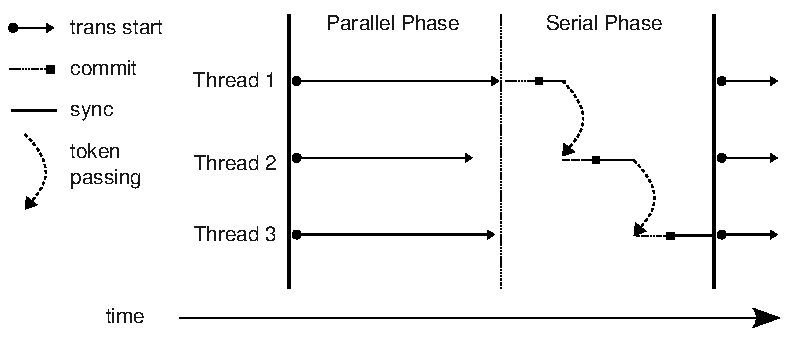
\includegraphics[width=3.25in]{dthreads/figure/phase}
\caption{An overview of \dthreads{} phase. Program execution with \dthreads{} alternates between parallel and serial phases.\label{fig:phase}}
}
\end{figure}

Figure~\ref{fig:phase} illustrates the execution of programs under \dthreads{}.  To guarantee determinism, \dthreads{} isolates memory accesses in parallel phases. In parallel phases, memory accesses work on private copies after the first write operation and updates are not shared across threads.  When a synchronization point is reached, updates are exposed in deterministic order.  This section describes the mechanisms used to guarantee deterministic commit order, and the details of commits to shared memory.

\subsubsection{Fence and Token}
\label{sec:schedule}

\dthreads{} places internal fences between the parallel and serial phases. \dthreads{} re-implements the fence because the standard \pthreads{} barrier mechanism does not support dynamic changes of threads number. 

\begin{figure}
\begin{lstlisting} [style=tt]
void waitFence(void) {
  lock();
	
  while(!isArrivalPhase()) { 
    CondWait();
  }

  waiting_threads++;
  if(waiting_threads < alive_threads) {
    while(!isDeparturePhase()) {
      CondWait();
    }
  } 
  else {
    setDeparturePhase();
    CondBroadcast();
  }

  waiting_threads--;
  if (waiting_threads == 0) {
    setArrivalPhase();
    CondBroadcast();
  }

  unlock();
}

\end{lstlisting}
\caption{Pseudocode for the internal fence.\label{fig:internalFence}}
\end{figure}

Figure~\ref{fig:internalFence} shows the pseudocode code for the internal fence. Threads must wait at the fence until all threads from the previous fence have departed. Then those threads are waiting on the fence until all alive threads  have entered into the same fence(lines 8-11). 
The last thread entering the fence initiates the departure phase and wakes up all threads on the fence(lines 14-15). As threads leave the fence, they decrement the waiting thread count.  The last thread to leave sets the fence to the arrival phase and wakes any waiting threads (lines 19-21).

To reduce overhead, whenever the number of running threads is
less than or equal to the number of cores, waiting threads block by spinning rather than by invoking relatively expensive cross-process \pthreads{} mutexes. When the number of threads exceeds the number of cores, \dthreads{} falls back to using \pthreads{} mutexes.

\begin{figure}
\begin{lstlisting} [style=tt]
void waitToken() {
  waitFence();
  while(isNotMyToken()) { yield(); }
}
void putToken() {
  passTokenToNextOfTokenQueue();
}
\end{lstlisting}
\caption{Pseudocode for waitToken and putToken. 
\label{fig:token}}
\end{figure}

Another key mechanism of \dthreads{} is using the token to order memory commits and synchronizations. The token implementation is listed in Figure~\ref{fig:token}. The token is a shared pointer that points to the next runnable thread entry, which guarantees the global order for all operations in serial phases.  

\dthreads{} introduces two subroutines to manage tokens.  The\texttt{waitToken()} function first waits at the internal fence and then waits to acquire the global token
in order to enter serial mode. The \texttt{putToken()} function passes the token to the next waiting thread. 

As shown in Figure~\ref{fig:phase}, it is very important for a thread to wait at the internal fence before a thread enters into serial phases or before a thread leaves serial phases, even for a thread that is guaranteed to have the token next. Memory commits by a thread can affect other threads' behavior. 

\subsubsection{Commit Protocol}
\begin{figure}
{\centering
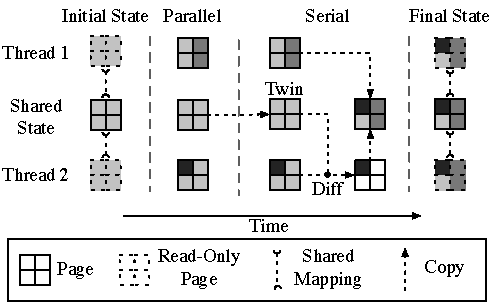
\includegraphics[width=5in]{dthreads/figure/architecture-diagram}
\caption{An overview of \dthreads{} execution.\label{fig:architecture}}
}
\end{figure}

Figure~\ref{fig:architecture} shows the steps to capture modifications to shared state and expose them in a deterministic order.  

At the beginning of the parallel phases, different threads have a read-only mapping for all shared pages. If a thread writes to a shared page during the parallel phases, this write is trapped in order to create a private copy and a twin page for this shared page. After that, reads and writes on this page happen on the private copy only. Reads go directly to the shared memory and are not trapped.  

In the serial phases, threads first commit their local changes happening in parallel phases one at a time, guided by the global token.  The first thread to commit to a page can directly copy its private copy to the shared state, but subsequent commits must copy only the modified bytes. To find out those modifications, \dthreads{} compares those private copies against those twin pages, creating from the shared mapping before actual modification.  After a thread commits its local changes, it issues synchronizations before it passes the token to next thread. 

In the end of serial phase, every threads have to wait at the fence in order to enter into the next parallel phase. 

\subsection{Deterministic Synchronization}
\label{sec:synchronization}
\dthreads{} supports the full range of synchronizations of
\pthreads{} APIs, including locks, conditional variables, barriers and different types of thread exit. Because the \sheriff{} framework can not provide any determinism guarantee, \dthreads{} re-implements all synchronizations as the following.

\subsubsection{Locks}
\dthreads{} uses the global token to guide synchronizations during the serial phases. Before a thread is acquiring a lock while current thread does not have the token, it has to wait for the global token. 

\dthreads{} treats multiple locks as the same one, which  possibly compromise the efficiency of programs, it only ends the serial phases when all locks are unlocked. Thus, it is possible for a program with deadlock problems that those deadlock do not occur to \dthreads{} at all. 

For the acquisitions of locks, \dthreads{} checks at first 
whether the current thread is already holding any locks. If not, the thread first waits for the token, commits those changes happened in the last parallel phase to shared state, and begins a new atomic section. Finally, the thread increments the number of locks it is currently holding. The lock count ensures that a thread does not pass the token to the next one until it has released all of the locks.

During the releases of locks, \dthreads{} decrements the lock count at first. A thread does nothing if there are still some locks holding by the current thread, with the lock count not equal to 0. If all locks have been released, \dthreads{} commits the memory changes happened in this serial phase to the shared mapping. Then it passes the global token to the next thread of the token queue and starts a new atomic region. Finally, the thread waits on the internal fence before entering into the next round's parallel phase.

\subsubsection{Condition Variables}
\label{sec:condwait}

Guaranteeing determinism for condition variables is much more complex than for other synchronization operations. The underlying operating system can not guarantee that threads are going to be waken-up in the same order as they wait on a conditional variable. Thus, a naive implementation easily leads to a deadlock problem.

% pthread_cond_wait: waiting threads are extracted from the 
% the token queue.
% Reducing the performance cost, 
When a thread calls \texttt{pthread\_cond\_wait}, it first acquires the global token and commits local modifications. It then removes itself from the token queue since threads waiting on condition variables do not participate in the token pass of the serial phase until they are awakened. Then, \dthreads{} adds itself to the conditional variable's waiting queue, decreases the alive thread count (used in the internal fence mechanism), and passes the token to the next thread on the token queue before actually waiting on a real process-shared conditional variable. When a thread is awaken, it should check at first whether the current thread is ready to run or not. For threads waken up by \texttt{pthread\_cond\_signal}, only the first thread in the waiting list can run in order to guarantee the First-In-First-Out order. All threads can run if waken up by \texttt{pthread\_cond\_broadcast}. If a thread is not able to run, it waits on the conditional variable again. If a thread is the candidate thread to be waken up, it waits for the global token because a thread waking up from a conditional variable is supposed to acquire the mutex, which means that it should already have the global token. 

For those waken-up functions, including \texttt{pthread\_cond\_signal} and \texttt{pthread\_cond\_broadcast}, the calling thread first waits for the token, and then commits any local modifications. If no threads are waiting on the condition variable, \dthreads{} passes the token to the next thread immediately. Otherwise, \dthreads{} moves corresponding threads in the condition variable queue to the head of the token queue, marked them as ready, and increments the live thread count correspondingly. To guarantee that threads are waken-up in the same order as they wait on a conditional variable, \texttt{pthread\_cond\_signal} only do this for the first thread in the queue but \dthreads{} wakes up all threads simultaneously. Those not-ready threads immediately wait again after waken-up. In order to improve the performance, those newly waken-up threads are scheduled to run next by simply putting them into the header of the token queue so that the calling thread can pass the token to them. 


\subsubsection{Barriers}

\label{sec:barrierwait}

\dthreads{} must ensure that threads waiting on a barrier do not disrupt the token passing of running threads. \dthreads{} removes threads entering into the barrier from the run queue and places them on the corresponding barrier queue.

In order to ensure the deterministic commit, the calling thread first waits for the global token to commit any local modifications. If the current thread is the last one to enter the barrier, \dthreads{} moves all threads on the barrier queue to the token queue, increases the alive threads count, and passes the token to the first thread in the barrier queue.  Otherwise, \dthreads{} removes the current thread from the token queue, places it on the barrier queue, releases the token. and waits on the actual barrier.


\subsubsection{Thread Creation and Exit}

\label{sec:threadcreation}

\begin{figure}
\begin{lstlisting} [style=tt]
void thread_create () {
  waitToken();
  clone(CLONE_FS| CLONE_FILES | CLONE_CHILD);
  if(isChild) {
    allocGlobalThreadIndex();
    insertToTokenQueue();
	notifyChildRegistered();
	// Wait for the parent to reach next sync point
    waitParentBroadcast();	
  }
  else if (isParent) {
    waitChildRegistered();
  }
}
\end{lstlisting}
\begin{lstlisting} [style=tt]
void thread_exit() {
  waitToken();
  atomicEnd(false);
  removeFromTokenQueue();
  decreaseInternalFence();
  putToken();
  exitThread(); 
}
\end{lstlisting}
\caption{Pseudocode for thread creation and exit($\S$~\ref{sec:threadcreation}).
\label{fig:threadcreation}
}
\end{figure}

To guarantee determinism, thread creation and exit must be performed in the serial phases.  Newly created threads are immediately added to the token queue.  For performance reason, the spawning thread does not immediately release the token until next different synchronization. This allows a single thread to quickly create multiple child threads without waiting for a new serial phase.

Figure~\ref{fig:threadcreation} shows pseudocode for thread creation and thread exit. The calling thread firstly waits for the token before proceeding (line 2).  It then creates a new process with shared file descriptors but a distinct address space using the \texttt{clone} system call (line 3).  The newly created child obtains the global thread index (line 5), places itself in the token queue (line 6), and notifies the parent that child has registered itself in the token queue(line 7). The child thread then waits for the parent to reach the next synchronization point. 

When \texttt{thread\_exit()} is called, the caller first waits for the token and then commits any local modifications (line 3). It then removes itself from the token queue (line 4) and decreases the number of threads required to proceed to the next phase (line 5). Finally, the thread passes its token to the next thread in the token queue (line 6) and exits (line 7).

\subsubsection{Thread Cancellation}

\dthreads{} implements the thread cancellation in serial phases in order to guarantee the determinism. phase. A thread can only invoke \texttt{pthread\_cancel} while holding the token. If the thread being cancelled is waiting on a condition variable or a barrier, it is removed from the queue deterministically. Finally, to cancel the corresponding thread, \dthreads{} kills the target process using kill(tid, SIGKILL) and the number of alive threads should be decremented after the cancellation.

\subsection{Deterministic Memory Allocation}
Programs sometimes rely on the addresses of objects returned by the memory allocator intentionally (for example, by hashing objects based on their addresses), or accidentally. A program with a memory error, like a buffer overflow, will yield different results for different memory layouts.

This reliance on memory addresses can undermine other efforts to provide determinism. For example, CoreDet is unable to fully enforce determinism because it relies on the Hoard scalable memory allocator~\cite{Bergan:2010:CCR:1736020.1736029}. Hoard was not designed to provide determinism and several of its mechanisms, thread id based hashing and non-deterministic assignment of memory to threads, lead to nondeterministic execution in CoreDet for the canneal benchmark.


To preserve determinism in the face of intentional or inadvertent reliance on memory addresses, we designed the \dthreads{} memory allocator to be fully deterministic. \dthreads{} assigns subheaps to each thread based on its thread index (deterministically assigned; see Section 4.1.2). In addition to guaranteeing the same mapping of threads to subheaps on repeated executions, \dthreads{} allocates superblocks (large chunks of memory) deterministically
by acquiring a lock (and the global token) on each
superblock allocation. Thus, threads always use the same subheaps, and these subheaps always contain the same superblocks on each execution. The remainder of the memory allocator is entirely deterministic. The superblocks themselves are allocated via mmap: while \dthreads{} could use a fixed address mapping for the heap, we currently simply disable ASLR to provide deterministic mmap calls. If a program does not use the absolute address of any heap object, \dthreads{} can guarantee determinism even with ASLR enabled.
Hash functions and lock-free algorithms frequently use absolute addresses, and any deterministic multithreading system must disable ASLR to provide deterministic results for these cases.


\section{Optimizations}
\label{sec:dthreads-optimization}

\dthreads{} performs a number of optimizations to improve performance.

\textbf{Lazy commit:} \dthreads{} reduces copying overhead and the time spent in the serial phase by lazily committing pages. When only one thread has ever modified a page, \dthreads{} considers that thread to be the page’s owner. An owned page is committed to shared state only when another thread attempts to read or write this page, or when the owner thread attempts to modify it in a later phase. \dthreads{} tracks reads with page protection and signals the owning thread to commit pages on demand. To reduce the number of read faults, pages holding global variables (which we expect to be shared) and any pages in the heap that have ever had multiple writers are all considered unowned and are not read-protected.

\textbf{Single-threaded-execution: }
When only one thread is running, \dthreads{} does not employ memory protection and treats all synchronization operations as no-ops. In addition, when only one thread is active because other threads are waiting on conditional variables, 
\dthreads{} does not try to commit local changes to the shared mapping (or discard private dirty pages). Updates are only committed when the thread issues a \texttt{cond\_signal} or \texttt{cond\_broadcast} call, which will wake up a thread and thus require publication of any updates.

\textbf{Lazy twin creation and diff elimination: }
Twin pages are only created when a page has multiple writers during the same phase. Also, \dthreads{} can commit its local changes by directly copying its working copy to the shared state, without performing a diff. This reduces the cost of a twin page allocation, a page copy, and a diff operation when a single thread is the exclusive writer of a page.

\textbf{Lock ownership:} \dthreads{} uses lock ownership to avoid unnecessary waiting when threads are using distinct locks. Initially, all locks are unowned. Any thread that attempts to acquire a lock that it does not own must wait until the serial phase to do so. If multiple threads attempt to acquire the same lock, this lock is marked as shared. If only one thread attempts to acquire the lock, this thread takes ownership of the lock and can acquire and release
it during the parallel phase. Lock ownership can result in starvation if one thread continues to re-acquire an owned lock without entering the serial phase. To avoid this, each lock has a maximum number of times it can be acquired during a parallel phase before a serial phase is required.

\textbf{Parallelization: }
\dthreads{} attempts to exploit as much parallelism as possible in the runtime system itself. One optimization is that at the start of transactions, \dthreads{} performs certain cleanup tasks, including releasing private page frames or resetting pages to read-only mode. It is safe to perform these cleanup tasks since these operations do not affect other the behavior of other threads.
Thus, \dthreads{} parallelizes a thread's cleanup tasks with other threads’ commit operations, without holding the global token. With this optimization, the token is passed to the next thread as soon as possible, saving time in the serial phase. 